\documentclass{beamer}
\beamertemplatenavigationsymbolsempty 

\title{WYSIWYG Stereo Painting}
\author{Dustin Ingram}
\institute{Interactive Computer Graphics, Spring 12-13\\ Drexel University
Department of Computer Science}
\date{\today}

\begin{document}
\maketitle

\begin{frame}
    \frametitle{The problem}
    \begin{itemize}
        \item 3D modeling is difficult and time-consuming;
        \item There are no adequate tools are available to-date to create artistic (non-photographic) stereo artwork from scratch;
    \end{itemize}
\end{frame}

\begin{frame}
    \frametitle{The goal}
    \begin{itemize}
        \item To answer the question, \emph{``What would a stereo Adobe Photoshop or Corel Painter look like?''};
        \item To create a what-you-see-is-what-you-get workflow for stereo painting;
    \end{itemize}
\end{frame}

\begin{frame}
    \frametitle{What is a stereo image?}
    \begin{itemize}
        \item 
        \item 
    \end{itemize}
\end{frame}

\begin{frame}
    \frametitle{An example of the process}
    The five steps necessary to create a Stereo Painting:
    \begin{figure}
        \centering
        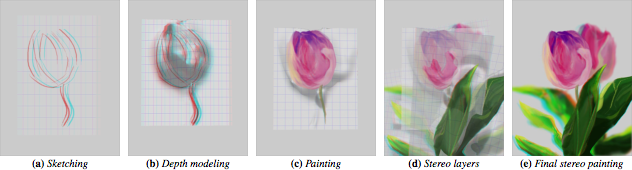
\includegraphics[width=0.8\paperwidth]{f1.png}
    \end{figure}
\end{frame}

\end{document}
